\chapter{Rešerše}
\label{1-reserse}

\section{Volba metody pro tvorbu webové aplikace}


Při volbě, jakou metodu pro tvorbu aplikace použít, se nabízely dvě
variant. První variantou by bylo použit skriptovací jazyka PHP a
druhou použít python framework pro tvorbu webových aplikací.

Hlavním faktorem při volbě metody zde byla úplná neznalost jazyka PHP,
se kterým jsem se během studia ani mimo něj nesetkal. Jasnou volbou
tedy bylo použití některého z python frameworků.

\section{Volba python frameworku}
Výběr vhodného frameworku po tvorbu aplikace byl vzhledem k jejich
množství opravdu složitý. Mezi hlavní kritéria pro výběr frameworku
jsme zařadili snadnou práce s databází, implementovat per object
permissions a dostupnost výukových materiálů a komunitní
podpora. Nakonec se vybíralo se ze dvou frameworků, a to Flask a
Django.

\begin{figure}[H] \centering
    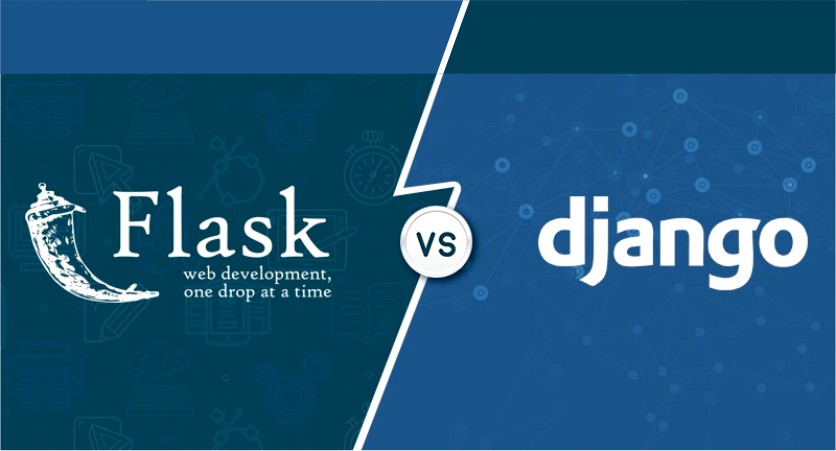
\includegraphics[width=240pt]{./pictures/1-django-vs-flask.jpeg}
    \caption[Flask vs Django]{Flask vs Django \cite{}}
	\label{fig:Flask vs Django}                                
\end{figure}

Flask je open source webový framework napsaný v Pythonu, klasifikovaný
jako mikro z důvodu, že není potřeba žádných dodatečných knihoven ani
jiných nástrojů. Do Flasku lze ovšem doinstalovat různá rozšíření,
která v základní verzi chybí jako například Flask-Admin, což je
administrátorské rozhraní pro správu uživatelů a objektů v
databázi. Výhodou je jeho velká obliba v komunitě, kdy v roce 2020 měl
druhé místo na GitHubu z webových frameworků, a díky tomu disponuje
spoustou materiálů a tutoriálů. Avšak velká nevýhoda flasku pro vývoj
naší aplikace je, že nedisponuje data modely. Pokud bychom v průběhu
vývoje chtěli přidat sloupec do naší databáze, musíme to udělat ručně
v databázi a poté ho přidat do třídy ve webové aplikaci.

Django je nejpoužívanějším open source frameworkem disponuje objektově
relačním mapováním. Jeho skvělou vlastností je tedy možnost generovat
model z databáze, který se zde může upravovat a poté jednoduchými
příkazy promítnout úpravy do databáze. Další výhodou je implementované
administrátorské rozhraní a možnost doinstalováním přídavných balíčků,
poskytující jak grafické úpravy, tak přidané funkce. Jedním z nich je
i balíček django-guardian zajišťující podporu per object permissions.

Z těchto dvou frameworků jsem nakonec vybral pro tvorbu aplikace
Django. To oproti Flasku disponovalo snadnou a rychlou práci s modelem
databáze. Další výhodou je vývojáři implementované administrátorské
rozhraní, které se nemusí doinstalovat pomocí přídavného balíčku. Z
hlediska popularity a dostupnosti výukových materiálu jsou na tom oba
frameworky podobně, kdy se oba řadí na první dvě místa výrazně před
ostatní frameworky.

\vspace{10px}

\section{Volba databáze}

Jedním z hlavních úkolů bylo vytvoření databáze, ze které se budou
zobrazovat poskytnutá data z projektu Viskalia, námi rozšířená o další
položky. Data zprostředkovaná Národním muzeem byla uložena v MySQL
databázi a jednalo se jak o textová, tak obrazová data uložena v
tabulkách. Příslušná databáze ovšem postrádá jakoukoli normalizaci a
data obsahují spoustu duplicit. Nabízí se proto otázka, zda provést
normalizaci dat a opět použít relační databázi, nebo použít nějakou z
nerelačních databází. Asi zásadní problém s NoSQL databází, který by
mohl nastat je problém v komunikaci s frameworkem pro vývoj webových
aplikací. Ty v zásadě nemají problém komunikovat s jakýmkoliv typem
relační databáze, ovšem často nemají engine pro databáze typu
NoSQL. Zvolili jsme tedy relační databázi a to MariaDB, která je
forkem původní MySQL. Od MySQL se liší pouze nepatrně a to přidanými
novými funkcemi, odstraněním bugů z MySQL a měla by zajišťovat
rychlejší operace s tabulkami.

\section{Automatizace deploymentu}

Jedním z hlavních úkolů je také automatizace deplymentu aplikace a
zajištění bezproblémového chodu na všech zařízeních. Při této otázce
jsme se nejprve museli rozhodnout, na jakém operačním systému se bude
aplikace vyvíjet a následně bude provozována. Po kratší úvaze jsme
zvolili systém Linux, který je vhodnější zejména pro vývoj aplikací v
jazyce Python. Zde jsme tedy hledali vhodný software pro
kontejnerizaci naší vyvíjené aplikace. Hlavními důvody pro jejich
použití je, že obsahují kompletní prostředí pro vývoj a chod aplikace
jako jsou knihovny nebo konfigurační soubory. Aplikace a všechny její
komponenty většinou běží v několika kontejnerech, které spolu dokáží
komunikovat. Jejich chod je od zbytku systému oddělen. Zde se nabízejí
dvě varianty, a to jsou LXC (LinuX Containers) anebo Docker, což jsou
jezdny z nejpoužívanějších aplikací. Hlavní rozdíl mezi těmito
aplikacemi je že kontejnery LXC obsahují svůj vlastní operační systém
a působí tedy spíše jako virtuální počítač. Docker oproti tomu žádné
takové prostředí nemá a běží pouze separovaně na operačním systému
uživatele. Dalším hlavním rozdílem je větší propracovanost Dockeru,
které umožňuje více nastavení kontejnerů a rozdělení aplikace do více
kontejnerů. Dalěím rozdílem oproti LXC je, že může být použit i na
jiném operačním systému než je linux. Z těchto důvodů byl pro
kontejnerizaci zvolen Docker.

\textbf{}
\textit{}



















